A classificação de pilares tem como objetivo considerar as diferentes situações de projeto e de cálculo, em relação aos esforços solicitantes em que cada um desses pilares se enquadra.

\begin{itemize}
	\item \textbf{Pilar intermediário}: Estão submetidos preponderantemente às forças axiais de compressão, pois os módulos dos momentos fletores são de pequena intensidade em relação às ações verticais apenas. Portanto, na situação de projeto, admite-se o pilar intermediário submetido a uma compressão centrada, isto é, a excentricidade inicial é considerada igual a zero para o dimensionamento das áreas das armaduras;

	\begin{figure}[H]
		\begin{center}
		\caption{Vista em planta de um pilar intermediário.}
    		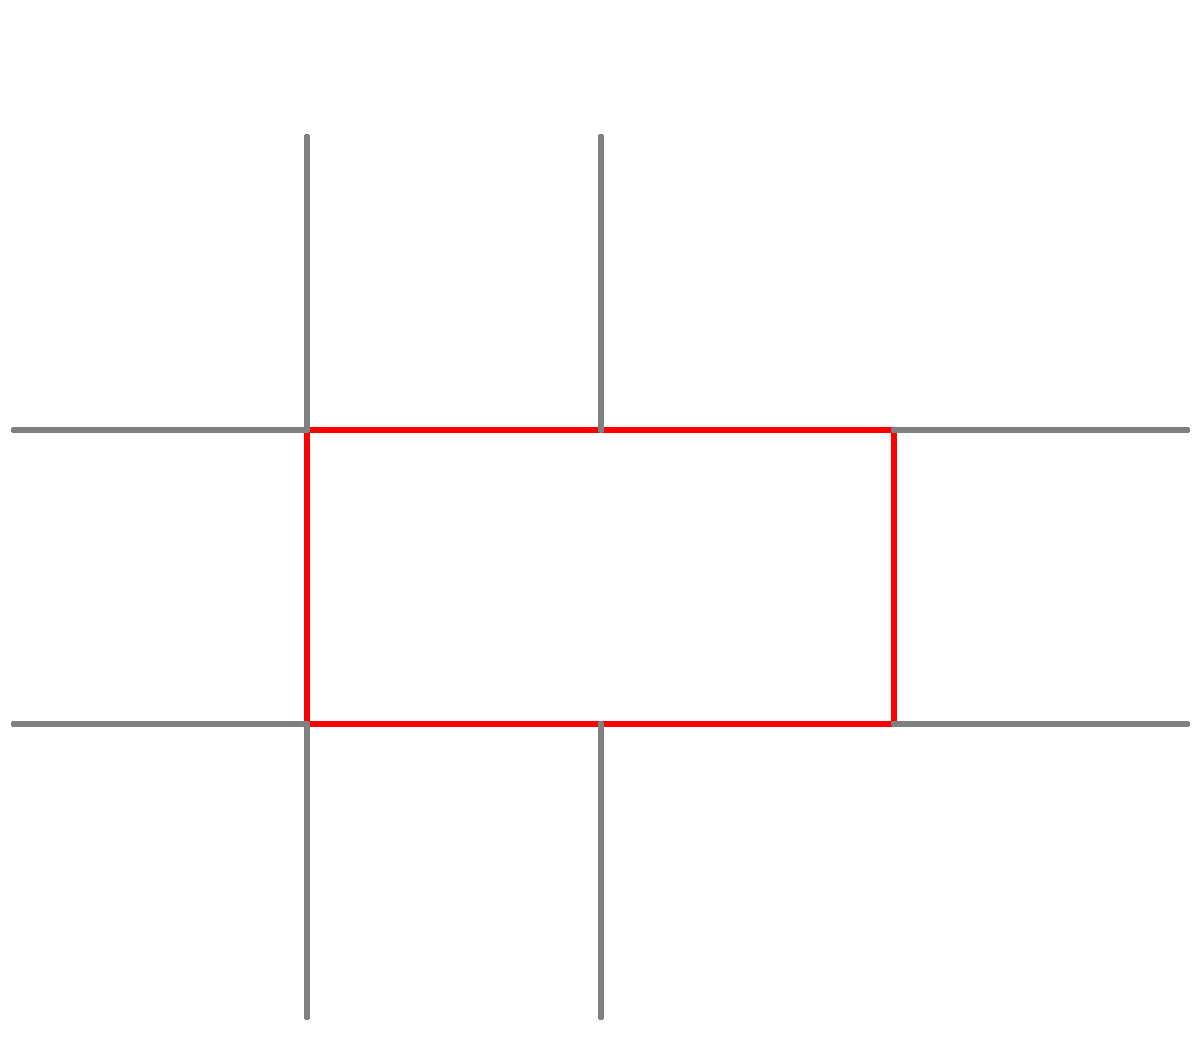
\includegraphics[width=0.3\textwidth]{Pilar-intermediario-de-extremidade-e-de-canto/Imagens/Pilar-intermediario.png}
		\end{center}
	\end{figure}

	\item \textbf{Pilar de extremidade}: Ficam posicionados nas bordas das edificações, sendo também chamados de laterais ou de borda. O termo "pilar de extremidade" advém do fato do pilar ser extremo para uma viga, aquela que não tem continuidade sobre o pilar. Além de estarem submetidos às forças normais de compressão, também estão sujeitos à ação de momentos transmitidos pelas vigas que têm suas extremidades externas nesses pilares. Portanto, na situação de projeto, admite-se o pilar de extremidade submetido à flexão normal composta, considerando-se excentricidade inicial segundo uma das coordenadas locais da seção tranversal do pilar;

	\begin{figure}[H]
		\begin{center}
		\caption{Vista em planta de um pilar de extremidade.}
    		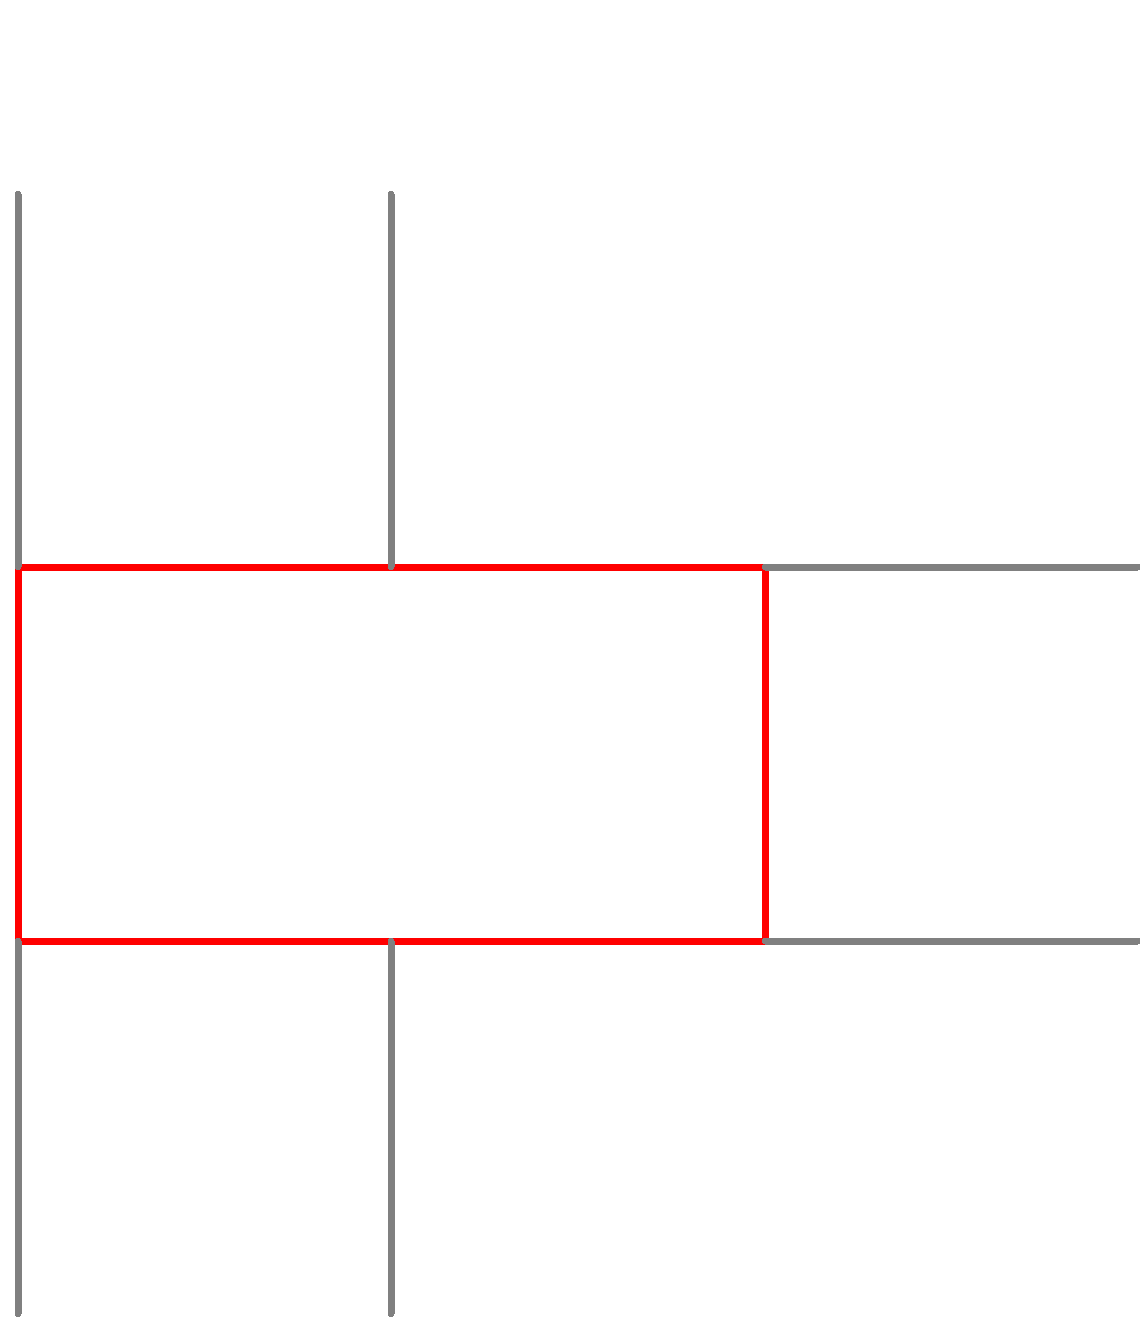
\includegraphics[width=0.2\textwidth]{Pilar-intermediario-de-extremidade-e-de-canto/Imagens/Pilar-de-extremidade.png}
		\end{center}
	\end{figure}

	\item \textbf{Pilar de canto}: Além da força normal de compressão atuante, consideram-se os momentos transmitidos pelas vigas, cujos planos médios são perpendiculares às faces dos pilares, e são interrompidas nas bordas do pilar. Na situação de projeto, considera-se o pilar de canto submetido à flexão obliqua composta, com excentricidades iniciais segundo os eixos coordenados locais.

	\begin{figure}[H]
		\begin{center}
		\caption{Vista em planta de um pilar de canto.}
    		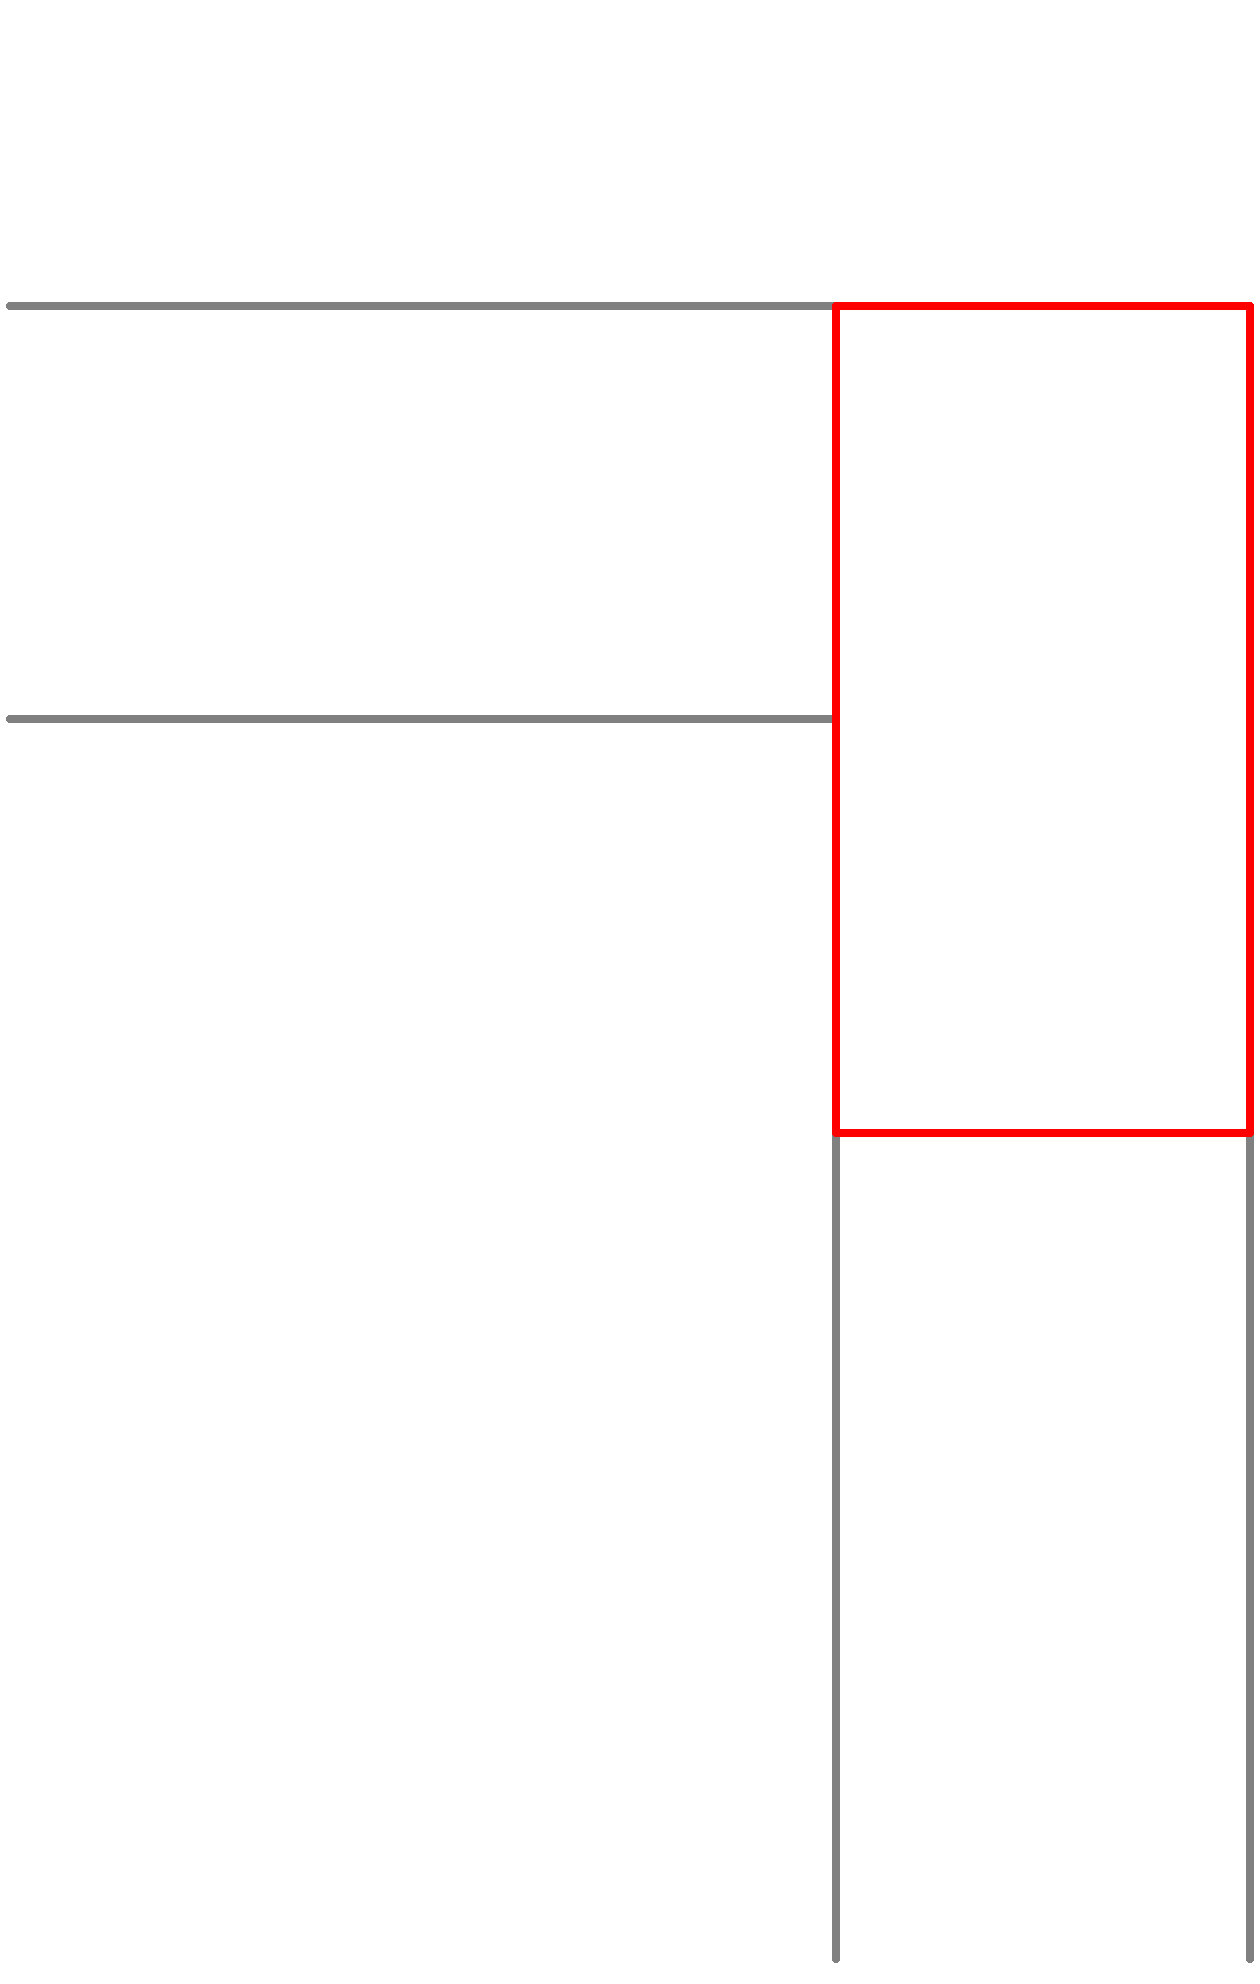
\includegraphics[width=0.2\textwidth]{Pilar-intermediario-de-extremidade-e-de-canto/Imagens/Pilar-de-canto.png}
		\end{center}
	\end{figure}

\end{itemize}